\documentclass[aspectratio=169]{beamer}
\usepackage{amsmath, amssymb, amsfonts, amsthm}
\usepackage{lmodern}
\usepackage{cancel}
\usepackage[output-complex-root=j]{siunitx}
\usepackage[american, nooldvoltagedirection]{circuitikz}
\usepackage{bm}
\usepackage{listings}
\usepackage{graphicx}
\usepackage{hyperref}

\usetheme{Berkeley}
\usefonttheme[onlymath]{serif}
\AtBeginSection[]{
    \begin{frame}
    \vfill
    \centering
    \begin{beamercolorbox}[sep=8pt,center,shadow=false,rounded=false]{title}
    \usebeamerfont{title}\insertsectionhead\par
    \end{beamercolorbox}
    \vfill
    \end{frame}
}

\newcommand{\N}{\mathbb{N}}
\newcommand{\Z}{\mathbb{Z}}
\newcommand{\Q}{\mathbb{Q}}
\newcommand{\R}{\mathbb{R}}
\renewcommand{\C}{\mathbb{C}}
\newcommand{\tpose}[1]{\left[#1\right]^{\! \top} \!\!}

\title{EECS 16B CSM}
\author{Bryan Ngo}
\date{2020-11-02}
\institute{UC Berkeley}

\begin{document}

\begin{frame}
    \maketitle
\end{frame}

\section{SVD}

\begin{frame}
    \frametitle{Definition}

    \begin{equation}
        \bm{A} = \sum_{i = 1}^r \sigma_i \bm{u}_i \tpose{\bm{v}_i} = \bm{U \Sigma} \tpose{\bm{V}} =
        \begin{bmatrix}
            \bm{u}_1 & \bm{u}_2 & \cdots & \bm{u}_r
        \end{bmatrix}
        \begin{bmatrix}
            \sigma_1 & 0 & \cdots & 0 \\
            0 & \sigma_2 & \cdots & 0 \\
            \vdots & \vdots & \ddots & \vdots \\
            0 & 0 & \cdots & \sigma_n
        \end{bmatrix}
        \begin{bmatrix}
            \tpose{\bm{v}_1} \\
            \tpose{\bm{v}_2} \\
            \vdots \\
            \tpose{\bm{v}_n}
        \end{bmatrix}
    \end{equation}
    \begin{itemize}
        \item \(\bm{U}\): orthonormal matrix
        \item \(\bm{\Sigma}\): diagonal matrix
        \item \(\tpose{\bm{V}}\): orthonormal matrix
    \end{itemize}
\end{frame}

\begin{frame}
    \frametitle{Visualization}

    \begin{center}
        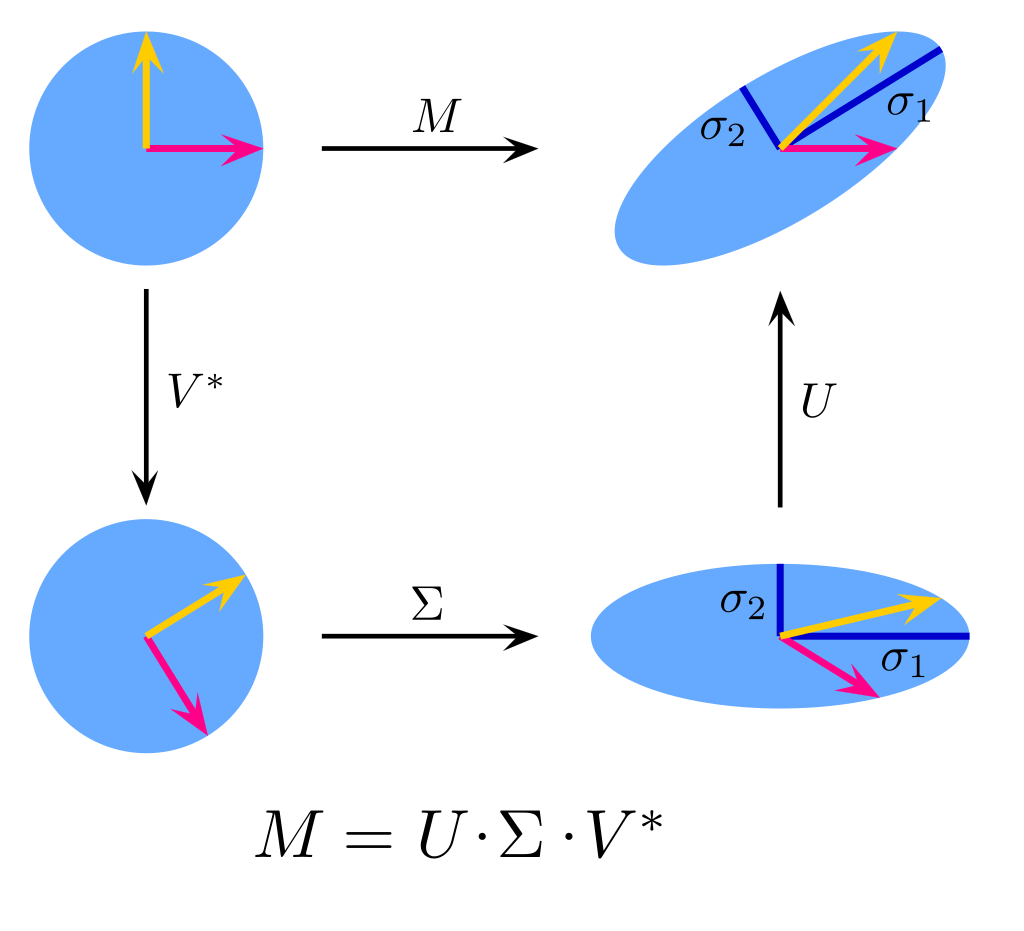
\includegraphics[height=0.9\textheight]{1024px-Singular-Value-Decomposition.svg.png}
    \end{center}
\end{frame}

\begin{frame}
    \frametitle{Gram-Schmidt Process}

    \begin{align}
        \bm{p}_i &= \bm{v}_i - \sum_{j = 1}^{i - 1} (\tpose{\bm{v}_i} \bm{w}_j) \bm{w}_j \\
        \bm{w}_i &= \frac{\bm{p}_i}{\|\bm{p}_i\|}
    \end{align}

    \begin{itemize}
        \item turns set of basis vectors to set of \emph{orthogonal} basis vectors
        \item systematically removing parallel components of our vector
    \end{itemize}
\end{frame}

\end{document}
